\section{Исследовательский раздел}

%1. Демонстрация работы ПО
%2. По возможности анализ результатов

\subsection{Технические характеристики}

Технические характеристики устройства, на котором запускалась программа, представлены ниже.
\begin{enumerate}
    \item Процессор: {AMD Ryzen 7 4700U} 2.0 ГГц~\cite{amd}, 8 физических ядер, 8 потоков;
    \item Оперативная память: 8 ГБ, {DDR4}, 3200 МГц;
    \item Операционная система: {Arch Linux}~\cite{arch};
    \item Версия ядра: {6.13.3}.
\end{enumerate}

Технические характеристики виртуальной машины QEMU~\cite{qemu}, на которой запускалась программа, представлены ниже.
\begin{enumerate}
    \item Виртуальная машина: qemu-system-x86\_64;
    \item Оперативная память: 2 ГБ;
    \item Операционная система: {Arch Linux};
    \item Версия ядра: {6.6} (собрано вручную с флагом CONFIG\_KALLSYMS=y и другими для возможности более глубокой отладки ядра).
\end{enumerate}

\subsection{Демонстрация работы ПО}

\begin{figure}[H]
	\centering
	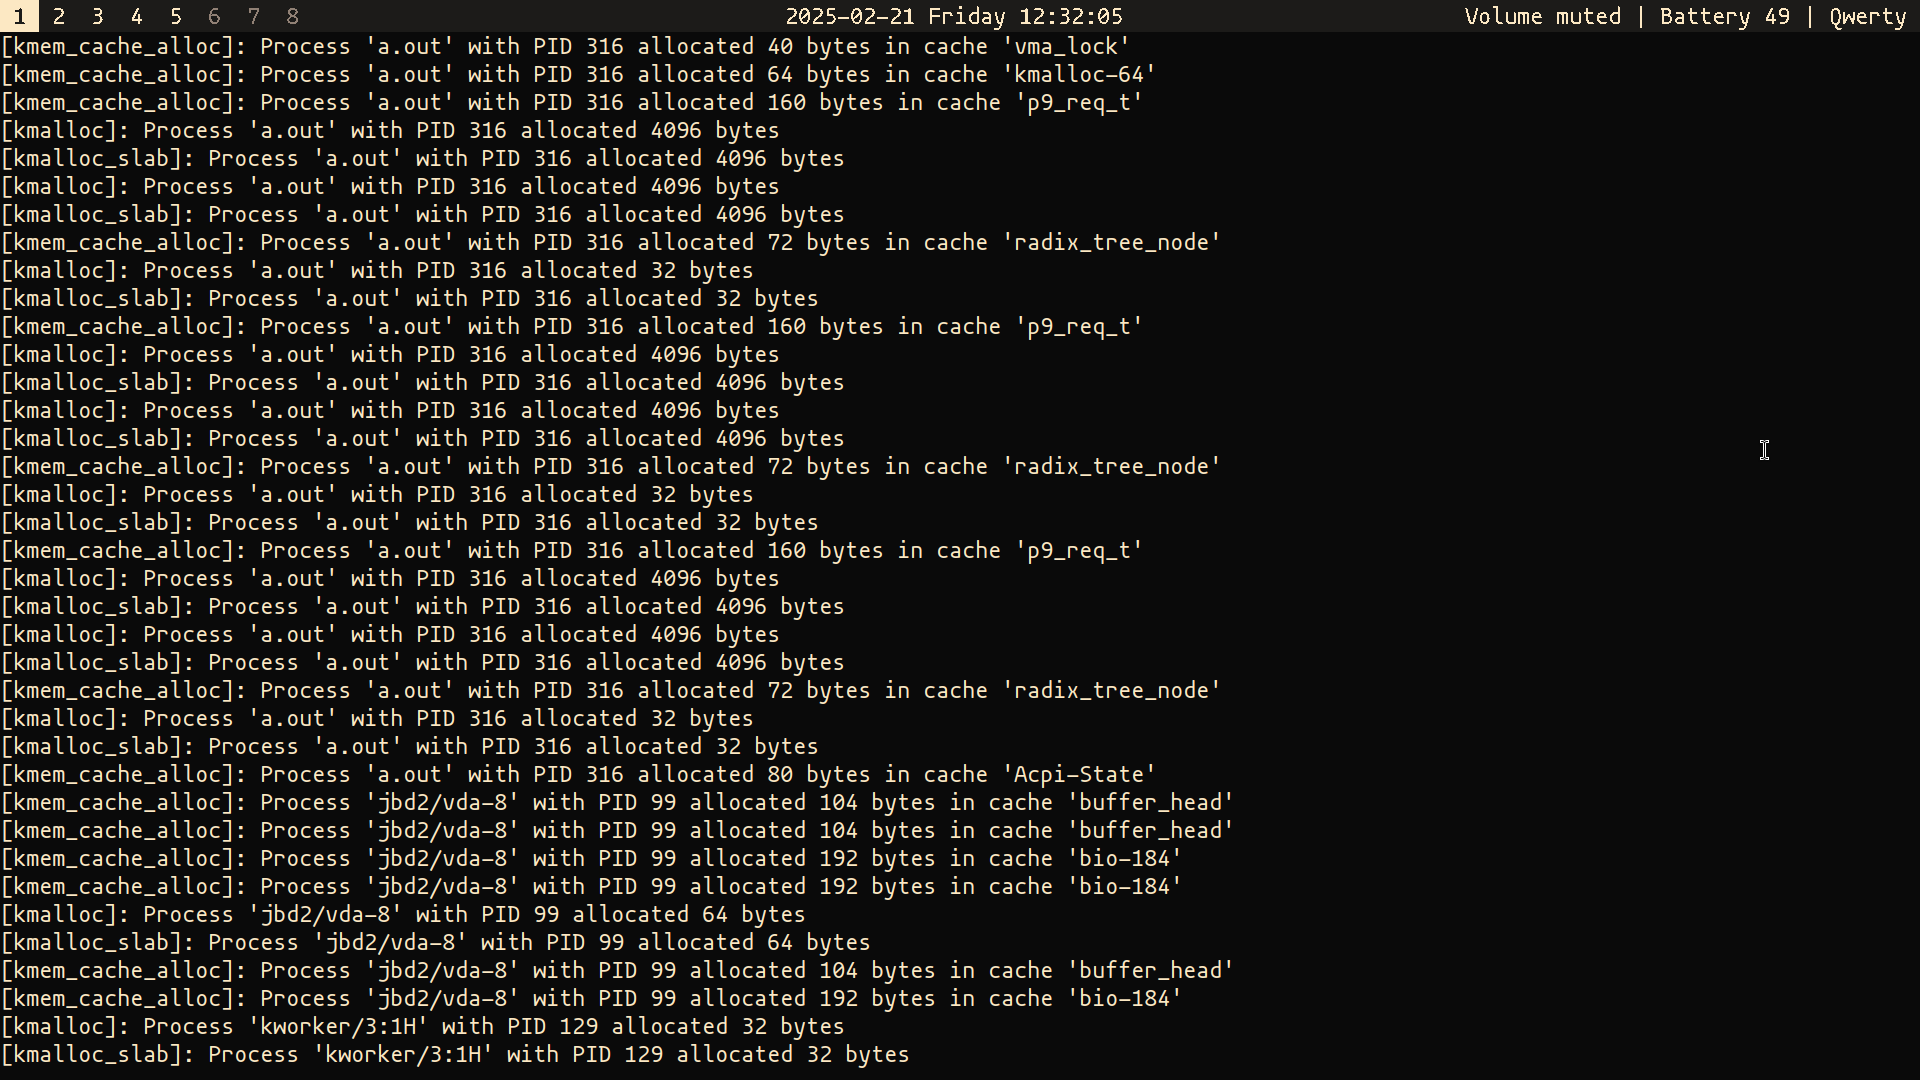
\includegraphics[width=0.9\textwidth]{img/out1.png}
	\caption{Демонстрация работы ПО 1}
	\label{fig:out1}
\end{figure}

\begin{figure}[H]
	\centering
	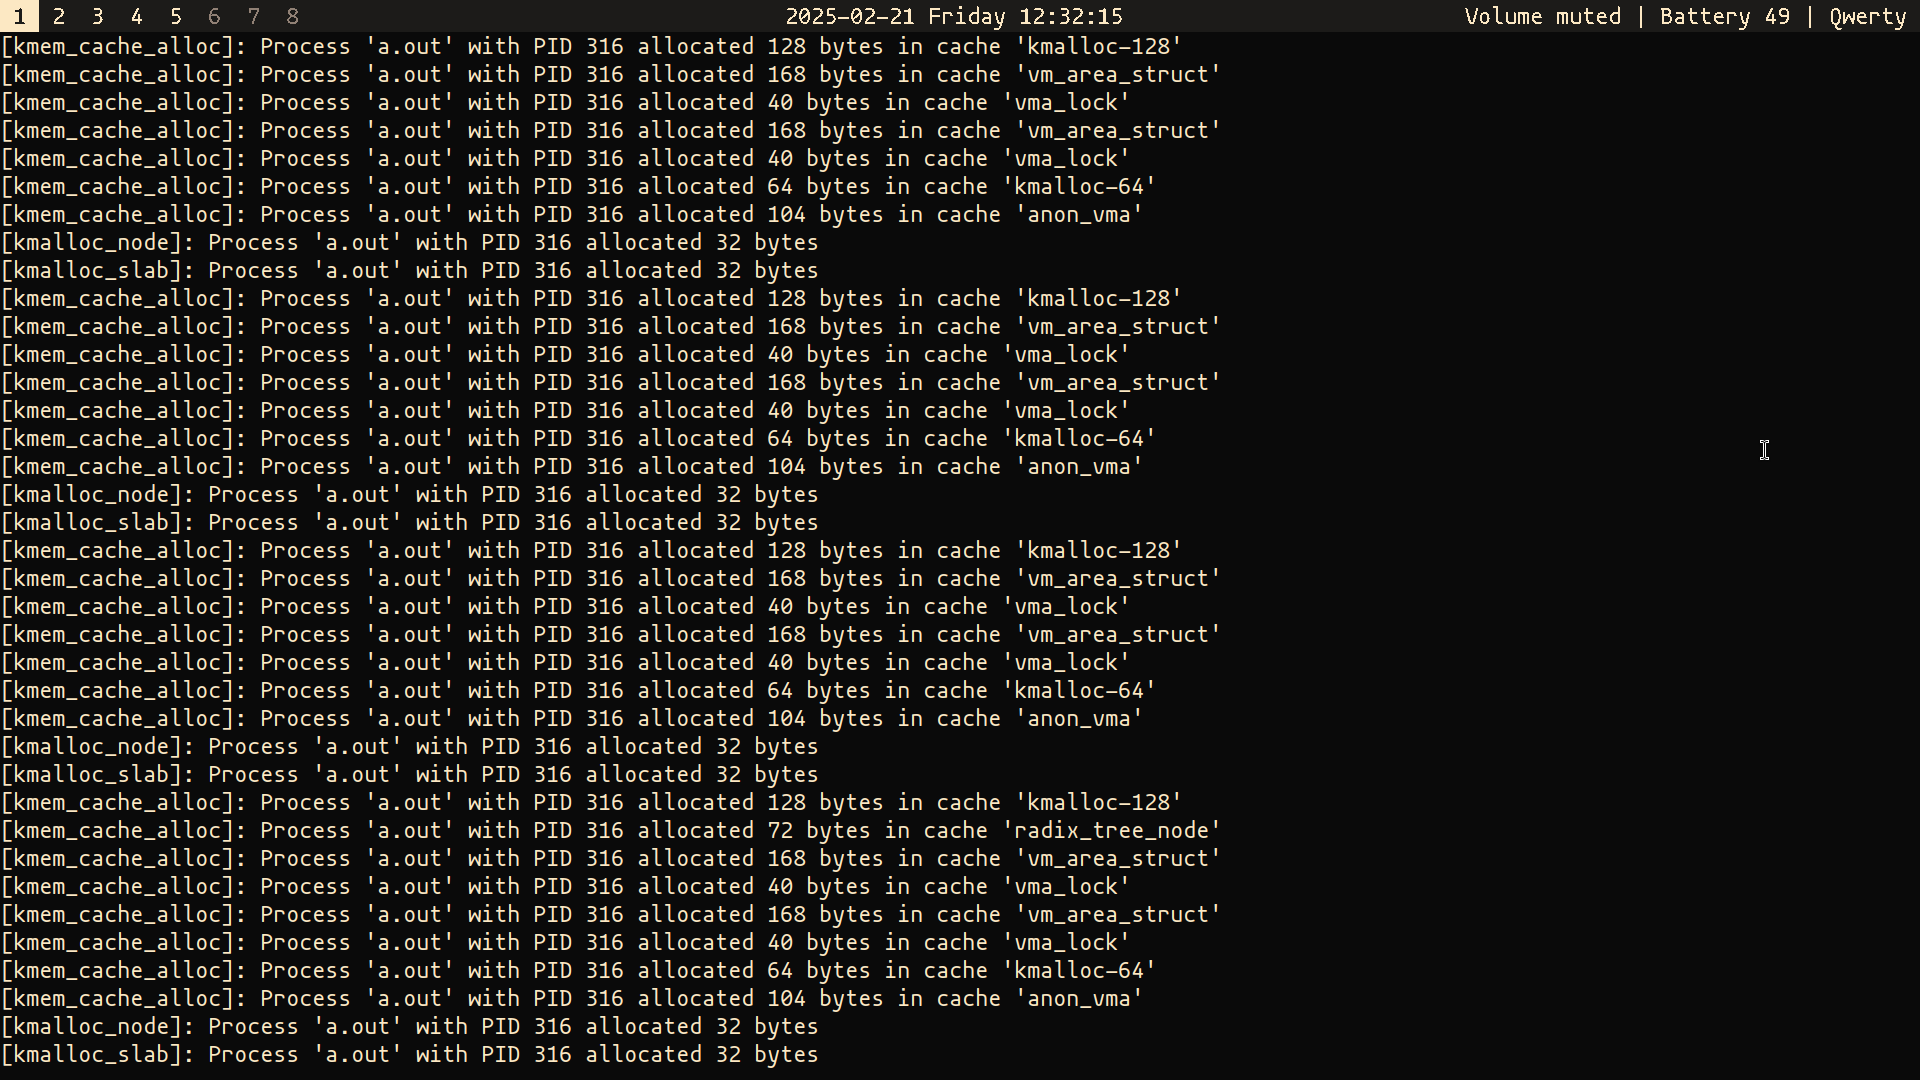
\includegraphics[width=0.9\textwidth]{img/out2.png}
	\caption{Демонстрация работы ПО 2}
	\label{fig:out2}
\end{figure}

\begin{figure}[H]
	\centering
	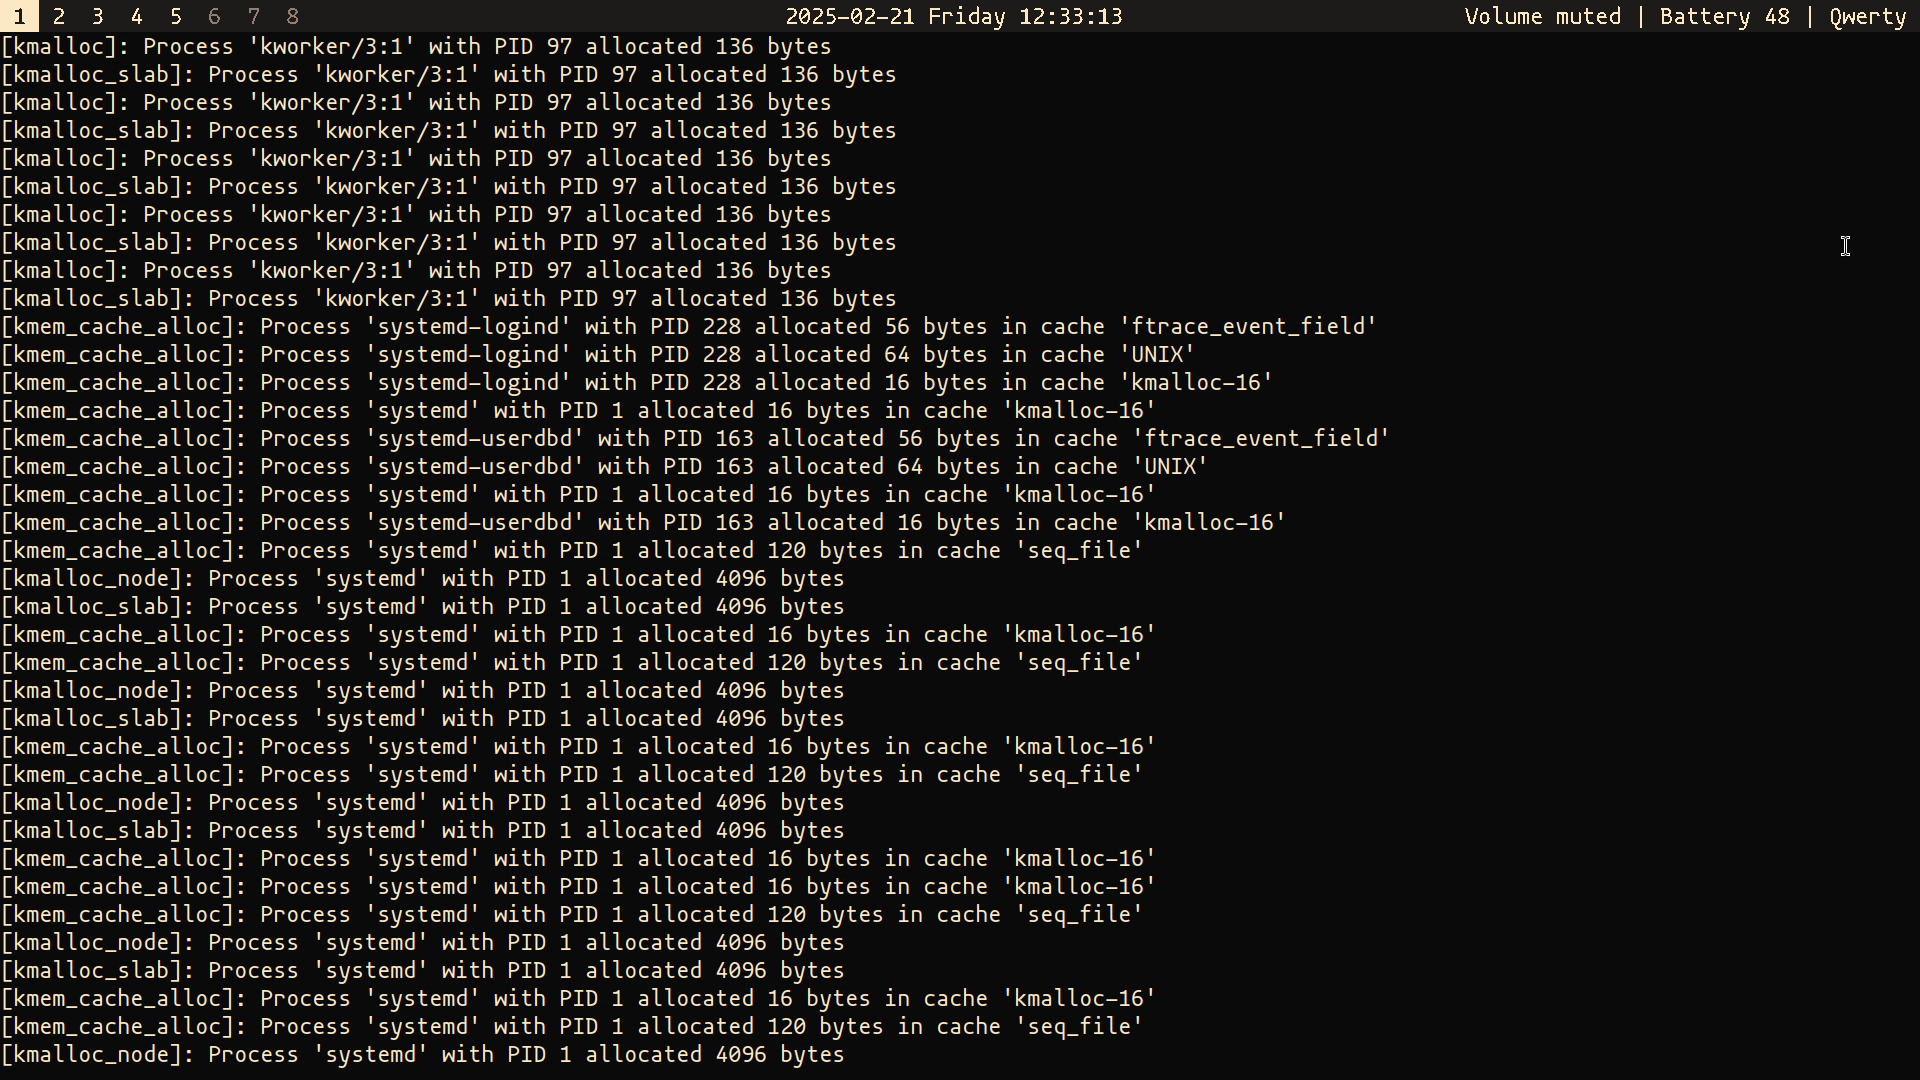
\includegraphics[width=0.9\textwidth]{img/out3.png}
	\caption{Демонстрация работы ПО 3}
	\label{fig:out3}
\end{figure}

\begin{figure}[H]
	\centering
	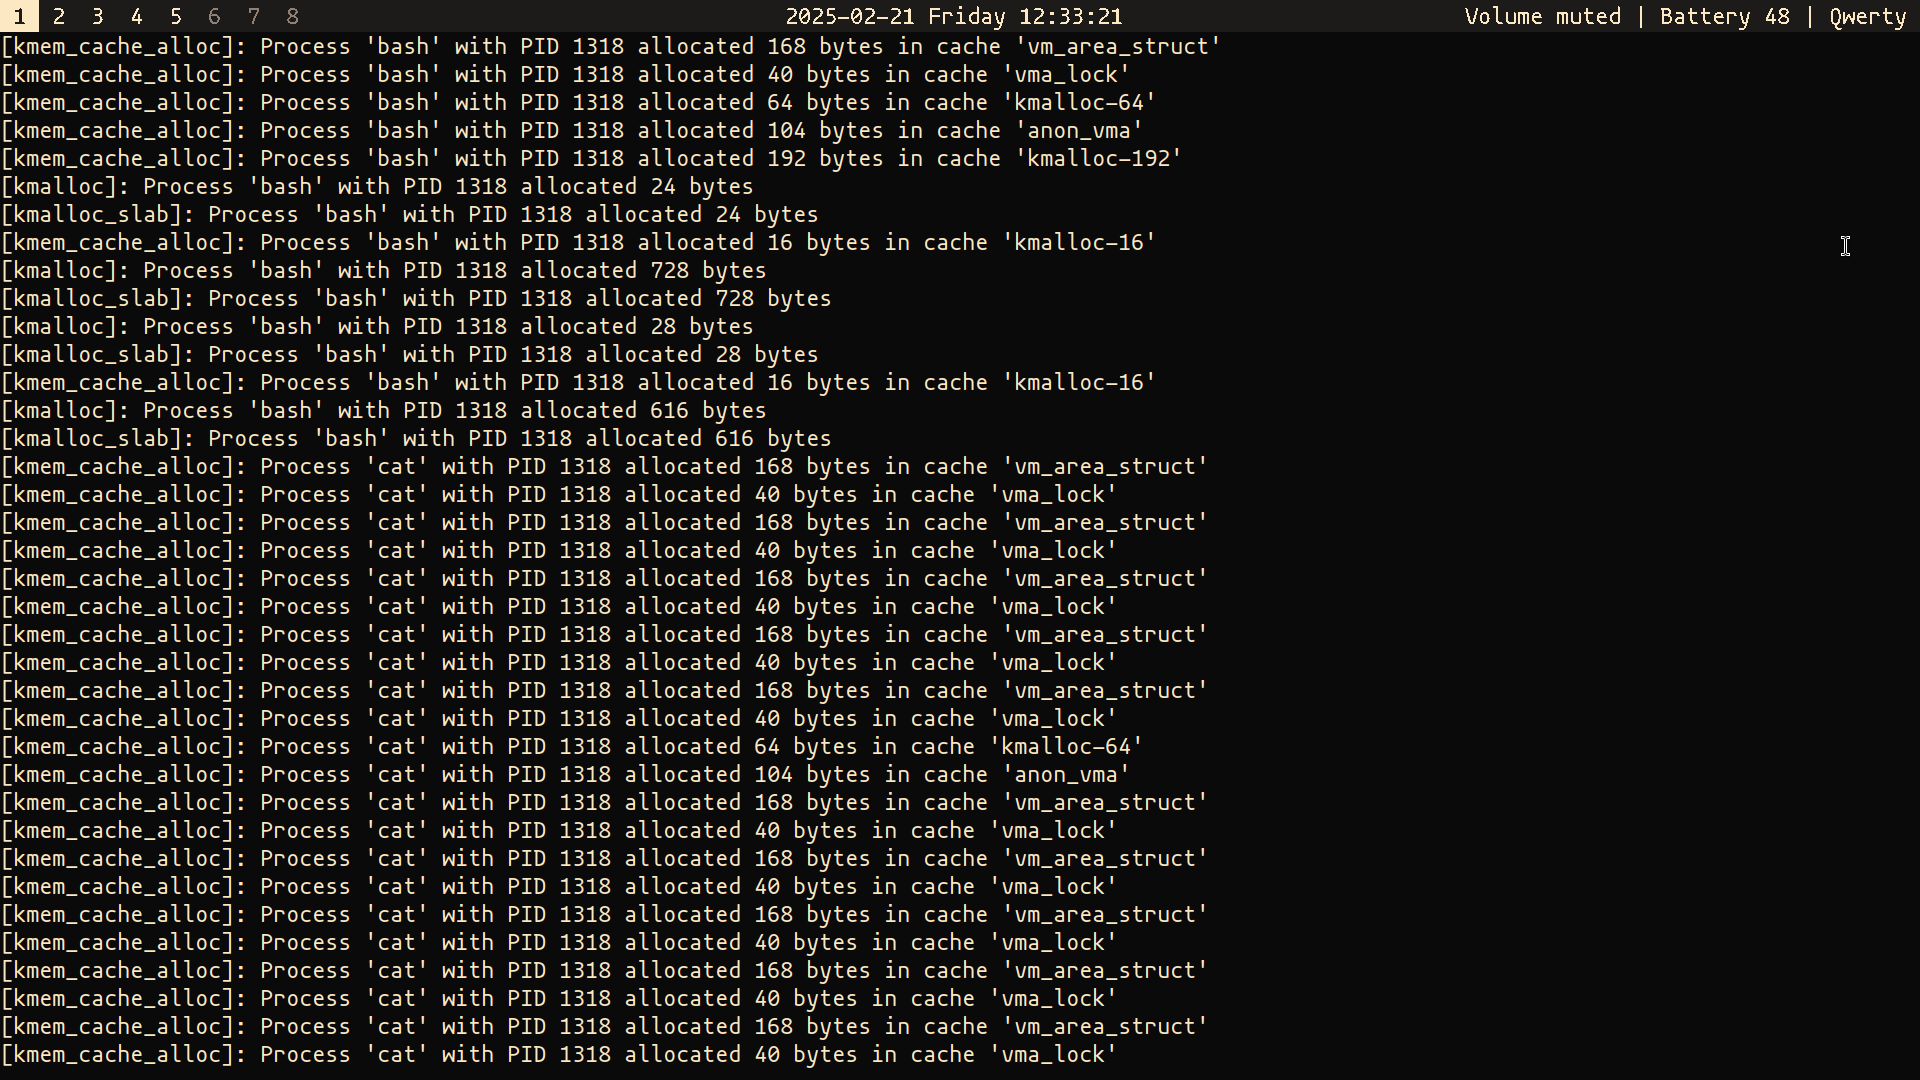
\includegraphics[width=0.9\textwidth]{img/out4.png}
	\caption{Демонстрация работы ПО 4}
	\label{fig:out4}
\end{figure}

\begin{figure}[H]
	\centering
	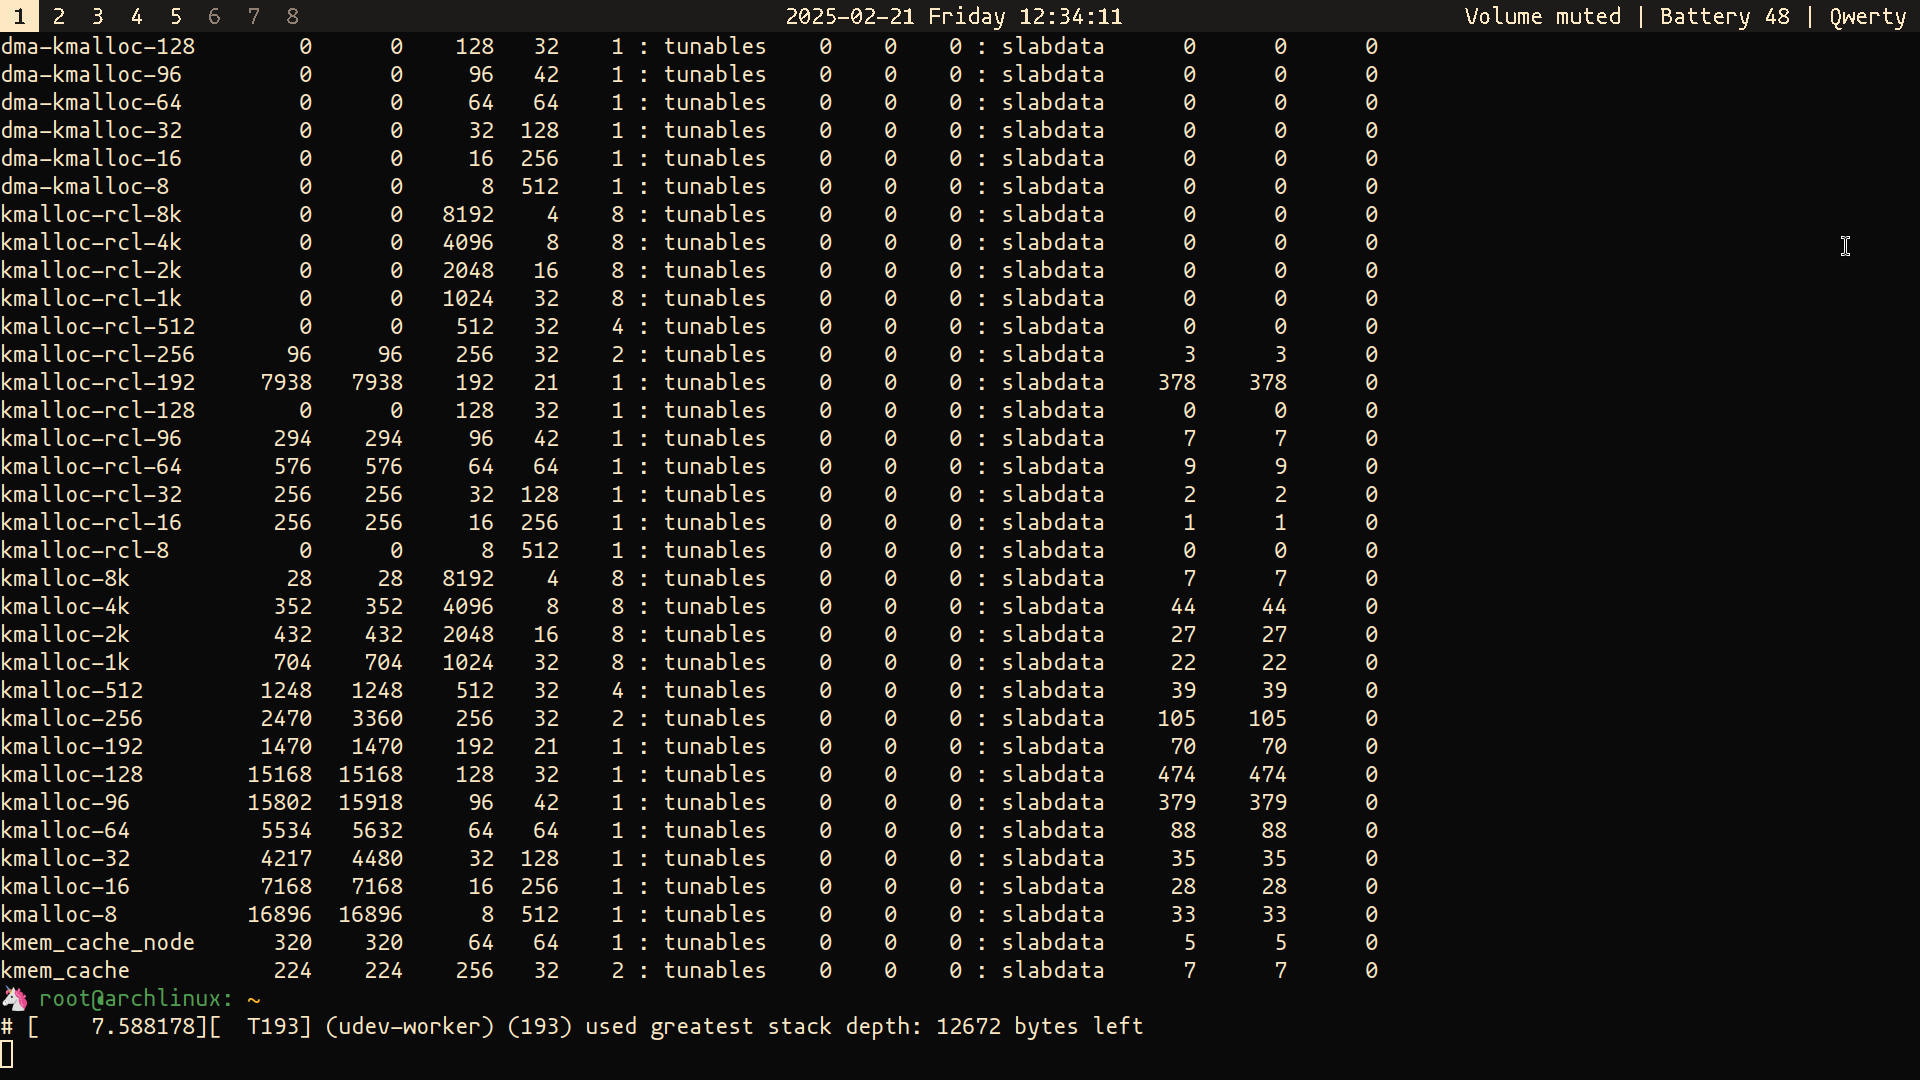
\includegraphics[width=0.9\textwidth]{img/slab-before.png}
	\caption{Вывод cat /proc/slabinfo до запуска программы для генерации потоков}
	\label{fig:slab-before}
\end{figure}

\begin{figure}[H]
	\centering
	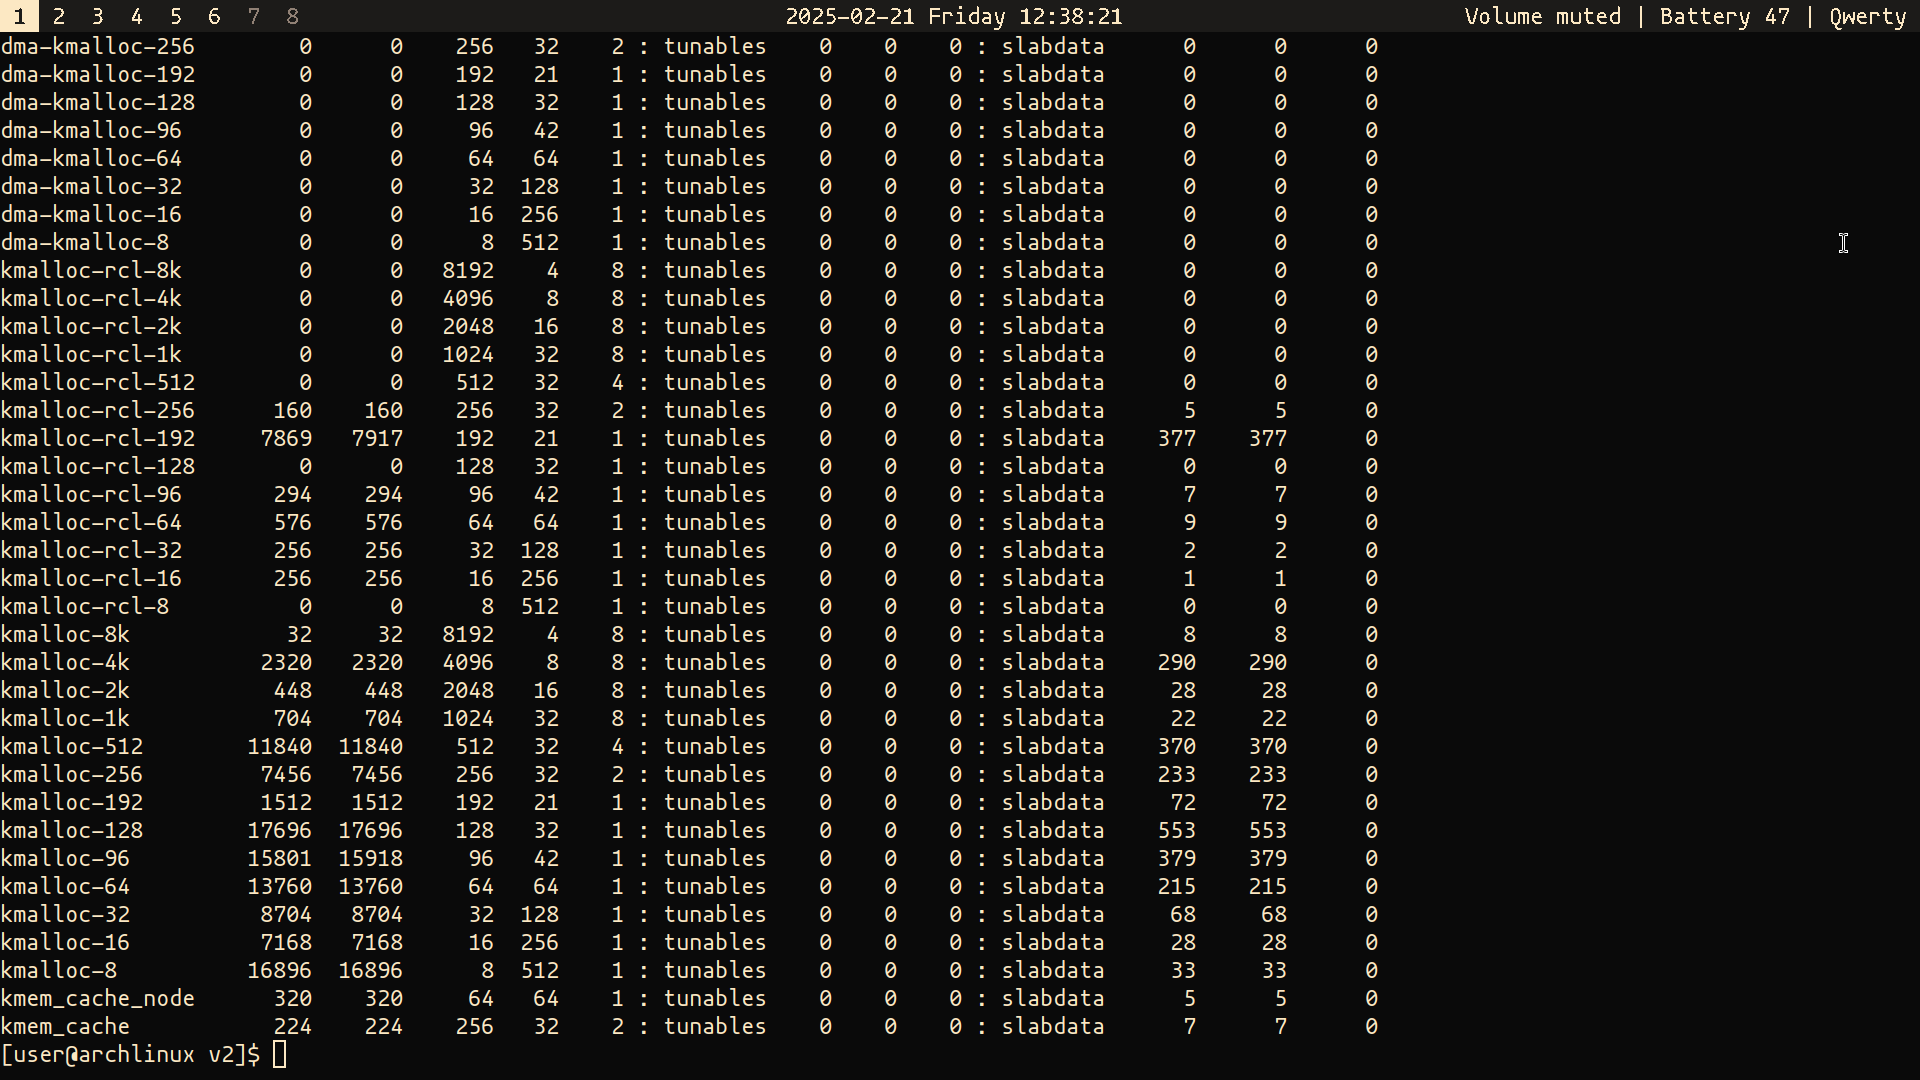
\includegraphics[width=0.9\textwidth]{img/slab-while.png}
	\caption{Вывод cat /proc/slabinfo во время запуска программы для генерации потоков}
	\label{fig:slab-while}
\end{figure}

\begin{figure}[H]
	\centering
	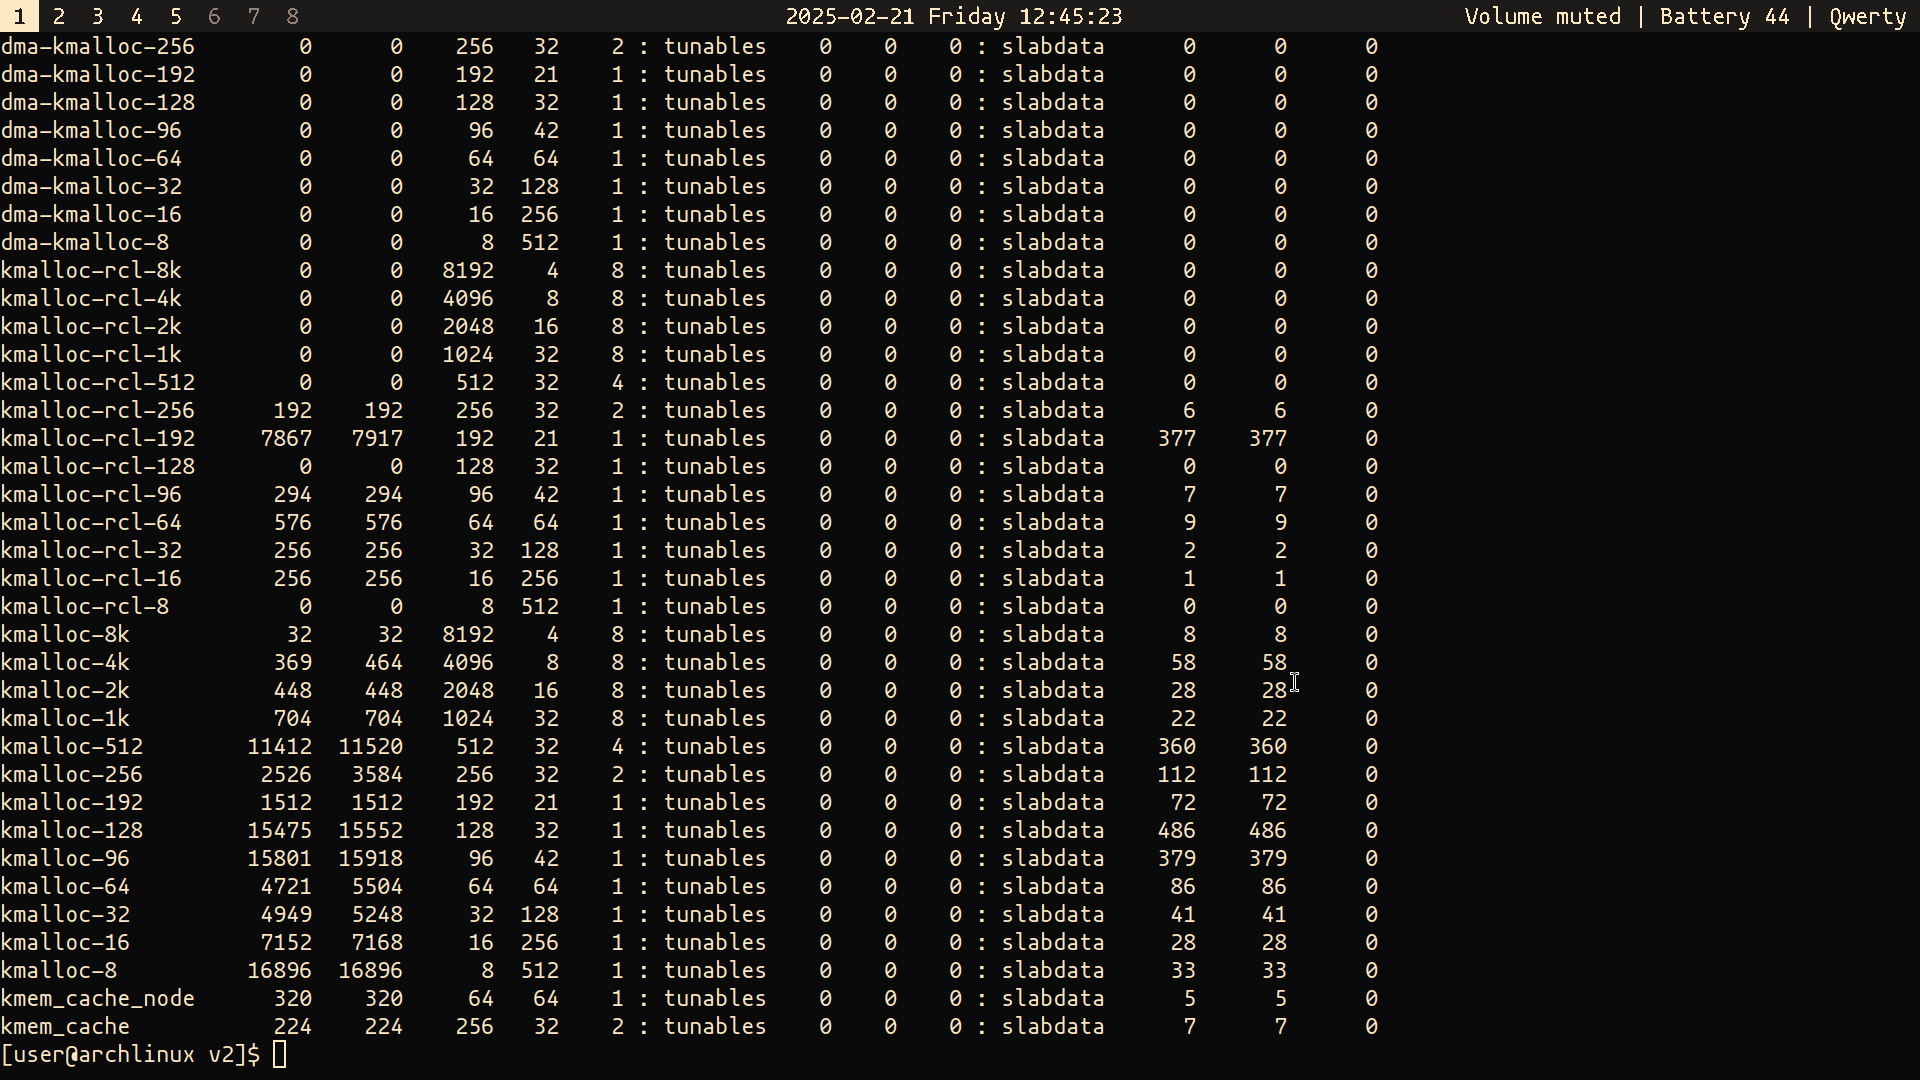
\includegraphics[width=0.9\textwidth]{img/slab-after.png}
	\caption{Вывод cat /proc/slabinfo после запуска программы для генерации потоков}
	\label{fig:slab-after}
\end{figure}

\newpage

\subsection{Анализ результатов работы ПО}

В таблице ниже представлено количество объектов в кэшах kmalloc-256, kmalloc-128 и kmalloc-64 соответственно до, во время и после запуска программы для генерации потоков.

\begin{table}[H]
    \centering
    \caption{Количество объектов в кэше}
    \label{tab:table}
    \begin{tabular}{|c|c|c|c|}
        \hline
        \,\hfill \textbf{Кэш} \hfill\, & \,\hfill \textbf{До} \hfill\, & \,\hfill \textbf{Во время} \hfill\, & \,\hfill \textbf{После} \hfill\, \\ \hline
        kmalloc-256 &  3360 &  7456 &  3584 \\ \hline
        kmalloc-128 & 15168 & 17696 & 15552 \\ \hline
        kmalloc-64  &  5632 & 13760 &  5504 \\ \hline
    \end{tabular}
\end{table}

Анализируя количество объектов в кэшах kmalloc-256, kmalloc-128 и kmalloc-64 до, во время и после запуска программы для генерации потоков, можно сделать вывод, что во всех трех кэшах наблюдается значительное увеличение количества объектов в период выполнения программы:
\begin{itemize}
    \item Наибольший рост зафиксирован в kmalloc-64 (на 144.3\%), что указывает на активное выделение небольших блоков памяти;
    \item В kmalloc-256 рост составил 121.9\%, что свидетельствует о значительном выделении памяти для относительно крупных объектов;
    \item В kmalloc-128 рост был менее выраженным (16.7\%), но также значительным.
\end{itemize}

\subsection*{Вывод}

В данном разделе были приведены технические характеристики устройства и виртуальной машины, на котором был запущен загружаемый модуль ядра, приведена демонстрация работы ПО, а также проведен анализ результатов его работы, в результате которого было зафиксировано увеличение количества выделяемых объектов в кэшах kmalloc-256, kmalloc-128, kmalloc-64.
